Un \textbf{protocolo de actualización de enrutamiento} es un mecanismo diseñado para permitir que los encaminadores (routers) intercambien información sobre la topología y el estado de la red de forma dinámica. Su función principal es \textbf{doble}: primero, permite calcular el conjunto de caminos más cortos hacia los destinos y, segundo, permite que la red responda ante fallos o cambios en la topología actualizando continuamente la información de las tablas.

Un principio rector en estos protocolos es que ninguno puede escalar lo suficiente como para permitir que todos los encaminadores de la Internet global intercambien información directamente; por ello, los encaminadores deben dividirse en grupos separados (Sistemas Autónomos) con protocolos que operen dentro de cada grupo. Hay tres razones principales por las cuales dividir los routers:

\begin{itemize}
	\item Trafico: Agregar más sitios a un protocolo aumenta exponencialmente el tráfico de enrutamiento.
	\item Comunicación indirecta: Muchos enrutadores en la Internet global están "lejos" entre sí y no comparten una red común, lo que imposibilita una comunicación directa y sencilla entre todos ellos.
	\item Limites administrativos: Internet no es gestionada por una sola entidad. Cada proveedor de servicios (ISP) o empresa quiere tener autonomía para controlar el enrutamiento y el acceso a sus redes de forma independiente. Además, las decisiones de ruta a menudo se basan en factores económicos y no solo en criterios técnicos
\end{itemize}

Aunque  es  deseable  que  los  routers  intercambien  información  de  enrutamiento, es  poco  práctico  para  todos  los  routers  en  una  Internet  arbitrariamente  grande,  participar  en  un  único  protocolo  de  actualización  de  enrutamiento.

A medida que el Internet crece, es imposible que un solo protocolo de enrutamiento gestione todos los routers del mundo. El "tamaño del grupo" (el número de routers que intercambian rutas) debe limitarse para evitar que las tablas de enrutamiento y el tráfico de actualización saturen la red. La solución es la jerarquía y la división del Internet en entidades menores llamadas Sistemas Autónomos. La determinación de cuántos enrutadores pueden participar en un grupo implica entender el tráfico generado, la capacidad de las redes y factores críticos de rendimiento. Existen dos cuestiones técnicas principales que limitan el tamaño de un grupo de enrutamiento:

\begin{itemize}
	\item Retraso (Tiempo de Convergencia): El interés principal no es el tiempo de propagación de un mensaje individual, sino el tiempo de convergencia, definido como el retraso máximo hasta que todos los enrutadores de la red son informados sobre un cambio en la topología
	\item Sobrecarga (Overhead): Dado que cada enrutador participante debe generar y enviar mensajes, un grupo más grande aumenta automáticamente el volumen de tráfico de enrutamiento
\end{itemize}

Debido a la dificultad de realizar un análisis técnico detallado en cada escenario, los administradores de red suelen seguir una pauta heurística basada en la experiencia:

\begin{itemize}
	\item En redes de área amplia (WAN): Se considera seguro permitir la participación de hasta una docena (12) de enrutadores en un único protocolo
	\item En redes de área local (LAN): El límite es aproximadamente cinco veces mayor (alrededor de 60 enrutadores), debido a la mayor capacidad y menor retardo de estas redes
\end{itemize}

Dado que las redes no son estáticas y el tráfico puede crecer por nuevas aplicaciones, los administradores implementan esquemas de monitoreo de tráfico. Mediante la escucha pasiva de la red, registran estadísticas sobre el porcentaje de ancho de banda consumido por los mensajes de enrutamiento frente al tráfico de datos durante periodos largos (semanas o meses) para decidir si es necesario subdividir los grupos de enrutadores.

Debido a que ningún protocolo de actualización de enrutamiento puede escalar de forma ilimitada, es necesario restringir el número de enrutadores que participan en un grupo de intercambio de información. Esta restricción técnica tiene una consecuencia arquitectónica inevitable: siempre habrá enrutadores que queden fuera del grupo participante.

El problema surge cuando un enrutador "no participante" intenta enviar datos utilizando a un miembro del grupo como su puerta de enlace (gateway) predeterminada.

Ejemplo típico: Considera tres enrutadores (R1, R2 y R3) conectados a una misma red troncal (backbone). R1 y R2 participan en el protocolo de enrutamiento y conocen todas las rutas, mientras que R3 es un "ajeno" que simplemente usa a R1 como su ruta por defecto.

La ineficiencia: Si R3 tiene un paquete para una red que está físicamente más cerca de R2, lo enviará primero a R1 a través de la red troncal. R1, al recibirlo, determinará que la mejor ruta es a través de R2 y enviará el paquete de vuelta por la misma red troncal hacia R2.

Resultado: El paquete realiza un viaje doble innecesario por la red troncal, consumiendo el doble de ancho de banda y recursos de los necesarios para llegar a su destino.

\begin{figure}[H]
	\centering
	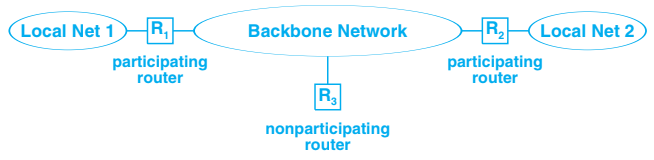
\includegraphics[width=0.8\textwidth]{img/backbone.png}
	\caption{Matriz de Encaminamiento central}
	\label{fig:grafico7}
\end{figure}

Este problema se puede clasificar como insidioso porque, a diferencia de un fallo total, el sistema parece funcionar correctamente: los datagramas llegan a su destino. Sin embargo, la red se vuelve extremadamente ineficiente sin que sea evidente a simple vista. Además, los mecanismos estándar de control como los mensajes de redirección ICMP no pueden solucionar esto, ya que estos mensajes solo se envían a la fuente original y no suelen ser procesados por enrutadores intermedios para corregir sus tablas de enrutamiento de forma dinámica.

\subsection{EGP (Exterior Gateway Protocol)}

El término Protocolo de Pasarela Exterior (EGP) se utiliza de manera genérica para designar cualquier protocolo empleado para transmitir información de accesibilidad de red entre dos Sistemas Autónomos (AS) distintos. En la arquitectura de Internet, un AS debe resumir la información de sus protocolos de actualización de rutas internos y propagar dicho resumen hacia el exterior a través de uno o más enrutadores configurados específicamente para esta tarea.

Estrictamente hablando, un EGP no es un protocolo de encaminamiento. La razón es que anunciar la accesibilidad (indicar simplemente que se puede llegar a una red a través de un AS) no es lo mismo que propagar información detallada de encaminamiento (como métricas de costo o topología interna). A pesar de esta distinción teórica, en la práctica profesional la mayoría de los expertos se refieren a los EGPs como protocolos de encaminamiento de forma indistinta

Para que un EGP cumpla su función, la información debe fluir en dos direcciones a través del enrutador fronterizo:

\begin{itemize}
	\item Hacia afuera: El enrutador recopila información sobre las redes dentro de su propio AS y la transmite al mundo exterior
	\item Hacia adentro: El enrutador acepta información sobre redes ubicadas en otros sistemas autónomos y difunde esa información de accesibilidad dentro de su propio AS
\end{itemize}

Aunque históricamente existieron otros protocolos, actualmente se utiliza un único protocolo de pasarela exterior para intercambiar información de accesibilidad en la Internet global: el Protocolo de Pasarela de Frontera (BGP). La versión utilizada hoy en día es la 4 (BGP-4), y es la herramienta que permite a los grandes Proveedores de Servicios de Internet (ISP) informarse mutuamente sobre los destinos a los que pueden llegar.

Cuando dos sistemas autónomos acuerdan intercambiar información utilizando BGP, cada uno designa un enrutador (llamado enrutador de borde o puerta de enlace de frontera) que hablará en su nombre. Estos dos dispositivos se convierten en pares BGP (BGP peers) entre sí y suelen estar conectados directamente en el límite físico de ambos sistemas.